\documentclass[aspectratio=169, 10pt]{beamer}

% ---------- Tema y colores ----------
\usetheme{default}
\usecolortheme{default}
\setbeamertemplate{navigation symbols}{}
\setbeamertemplate{footline}[frame number]
\setbeamertemplate{frametitle continuation}{}

\definecolor{StanfordRed}{RGB}{140,21,21}
\definecolor{StanfordGray}{RGB}{77,77,77}
\definecolor{LightGray}{RGB}{240,240,240}
\definecolor{AccentBlue}{RGB}{0,84,166}
\definecolor{AccentGreen}{RGB}{0,130,100}
\definecolor{UCMBlue}{RGB}{4, 171, 226}
\definecolor{UCMNavy}{RGB}{20, 65, 134}

% Alias de la paleta antigua: las figuras TikZ de esta clase siguen
% usando mitblue/mitgray, que ahora apuntan a los colores UCM.
\definecolor{mitblue}{RGB}{20, 65, 134}
\definecolor{mitgray}{RGB}{169, 169, 169}

\setbeamercolor{frametitle}{fg=white, bg=UCMBlue}
\setbeamercolor{title}{fg=white}
\setbeamercolor{author}{fg=white}
\setbeamercolor{institute}{fg=white!80}
\setbeamercolor{structure}{fg=UCMBlue}
\setbeamercolor{block title}{bg=UCMBlue!15!white, fg=UCMBlue}
\setbeamercolor{block body}{bg=LightGray}
\setbeamercolor{block title alerted}{bg=StanfordRed!15!white, fg=StanfordRed}
\setbeamercolor{block body alerted}{bg=LightGray}
\setbeamercolor{block title example}{bg=AccentGreen!15!white, fg=AccentGreen}
\setbeamercolor{block body example}{bg=LightGray}
\setbeamercolor{alerted text}{fg=UCMBlue}
\setbeamercolor{example text}{fg=UCMBlue}

\setbeamerfont{frametitle}{series=\bfseries, size=\large}
\setbeamerfont{title}{series=\bfseries, size=\LARGE}
\setbeamerfont{block title}{series=\bfseries}

% ---------- Paquetes ----------
\usepackage[utf8]{inputenc}
\usepackage[T1]{fontenc}
\usepackage[provide=*,spanish]{babel}
\usepackage{amsmath, amssymb, bm}
\usepackage{graphicx}
\usepackage{tikz}
\usepackage{pgfplots}
\pgfplotsset{compat=1.18}
\usetikzlibrary{arrows, arrows.meta, shapes, shapes.geometric, positioning,
	fit, calc, matrix, chains, mindmap, decorations.pathreplacing,
	backgrounds, shadows, patterns}
\usepackage{booktabs}
\usepackage{xcolor}
\usepackage{multicol}
\usepackage{ragged2e}
\usepackage{tcolorbox}
\tcbuselibrary{skins, breakable}


% ---------- Comandos útiles ----------
\providecommand{\R}{\mathbb{R}}
\providecommand{\E}{\mathbb{E}}
\providecommand{\Var}{\operatorname{Var}}
\providecommand{\relu}{\operatorname{ReLU}}

\newcommand{\formula}[1]{%
	\begin{tcolorbox}[colback=UCMBlue!8, colframe=UCMBlue, arc=4pt,
		boxsep=2pt, left=6pt, right=6pt, top=3pt, bottom=3pt]
		#1
	\end{tcolorbox}
}

% Caja para la lectura de un diagrama
\newcommand{\idea}[1]{%
	\begin{tcolorbox}[colback=AccentGreen!6, colframe=AccentGreen, arc=3pt,
		width=\textwidth, boxsep=1pt, left=5pt, right=5pt, top=2pt, bottom=2pt,
		fontupper=\small]
		\RaggedRight\textbf{Idea clave:} #1
	\end{tcolorbox}
}

% Marca de procedencia de una figura o dato
\newcommand{\fuente}[1]{{\scriptsize\color{StanfordGray}#1}}

% ---------- Portada ----------
\title{\textbf{¿Por qu\'e funciona el aprendizaje profundo?}}
\subtitle{Sobreparametrizaci\'on, paisaje de p\'erdida y generalizaci\'on}
\author{Sergio Hern\'andez, PhD\\ shernandez@ucm.cl}
\institute{
	\begin{tikzpicture}[scale=0.42, every node/.style={transform shape}]
		\foreach \i/\y in {1/0,2/1,3/2}{\node[circle,draw=white,fill=white!20,minimum size=4mm] (i\i) at (0,\y){};}
		\foreach \i/\y in {1/-0.5,2/0.5,3/1.5,4/2.5}{\node[circle,draw=white,fill=white!35,minimum size=4mm] (h\i) at (2,\y){};}
		\foreach \i/\y in {1/0.5,2/1.5}{\node[circle,draw=white,fill=white!50,minimum size=4mm] (o\i) at (4,\y){};}
		\foreach \a in {1,2,3}\foreach \b in {1,2,3,4}{\draw[white,opacity=0.5] (i\a)--(h\b);}
		\foreach \a in {1,2,3,4}\foreach \b in {1,2}{\draw[white,opacity=0.5] (h\a)--(o\b);}
	\end{tikzpicture}
	\\ \textbf{Mag\'ister en Data Science --- Universidad Cat\'olica del Maule}}
\date{}


\begin{document}
% --- Título ---
{
	\setbeamertemplate{background}{
		\begin{tikzpicture}[remember picture, overlay]
			\fill[UCMBlue] (current page.south west) rectangle (current page.north east);
			\fill[UCMBlue!70!black, opacity=0.5]
			(current page.south west) -- ++(0,3) -- ++(18,0) -- cycle;
			\foreach \i in {1,...,40}{
				\fill[white, opacity=0.04]
				({random()*17}, {random()*10}) circle ({random()*0.3});
			}
		\end{tikzpicture}
	}
	\begin{frame}[plain]
		\vspace{1.2cm}
		\titlepage
		\begin{tikzpicture}[remember picture, overlay]
			\node[white, opacity=0.15, font=\fontsize{80}{80}\selectfont]
			at (current page.east) [xshift=-2cm] {?};
		\end{tikzpicture}
	\end{frame}
}


\begin{frame}
\frametitle{Hoja de ruta}
\begin{columns}[T]
\begin{column}{6cm}
\begin{enumerate}
	\item El caso \emph{en contra} del aprendizaje profundo
	\item Qu\'e hace f\'acil el ajuste
	\item C\'omo es el paisaje de la funci\'on de p\'erdida
\end{enumerate}
\end{column}
\begin{column}{6cm}
\begin{enumerate}
	\setcounter{enumi}{3}
	\item Qu\'e determina la generalizaci\'on
	\item ¿Hacen falta tantos par\'ametros?
	\item ¿Tienen que ser profundas?
\end{enumerate}
\end{column}
\end{columns}
\vspace{0.8em}
\begin{block}{Objetivo de la clase}
Esta clase no presenta resultados establecidos: presenta \textbf{preguntas abiertas}. Hasta aqu\'i vimos \emph{c\'omo} se construyen y entrenan las redes; hoy preguntamos \textbf{por qu\'e eso funciona} --- y hasta d\'onde llega realmente nuestra comprensi\'on.
\end{block}
\vspace{0.3em}
\fuente{Basado en Prince, \emph{Understanding Deep Learning}, cap.~20.}
\end{frame}

%=====================================================================
\section{El caso en contra del aprendizaje profundo}
%=====================================================================

\begin{frame}
\frametitle{A priori, esto no debería funcionar}
\begin{center}
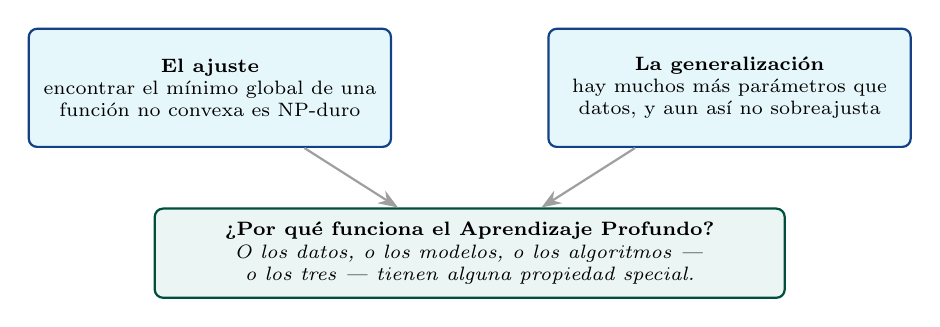
\begin{tikzpicture}[font=\scriptsize,
	caja/.style={rectangle, rounded corners=3pt, draw=UCMNavy, thick,
		fill=UCMBlue!10, minimum width=4.6cm, minimum height=1.5cm,
		align=center, inner sep=4pt},
	fl/.style={-{Stealth[length=2.5mm]}, thick, gray!75}]

	\node[caja] (a) at (0,0)
		{\textbf{El ajuste}\\
		 encontrar el m\'inimo global de una\\ funci\'on no convexa es NP-duro};
	\node[caja] (b) at (6.6,0)
		{\textbf{La generalizaci\'on}\\
		 hay muchos m\'as par\'ametros que\\ datos, y aun as\'i no sobreajusta};

	\node[rectangle, rounded corners=3pt, draw=AccentGreen!60!black, thick,
		fill=AccentGreen!8, minimum width=8cm, align=center, inner sep=5pt]
		(c) at (3.3,-2.1)
		{\textbf{¿Por qu\'e funciona el Aprendizaje Profundo?}\\
		 \emph{O los datos, o los modelos, o los algoritmos ---}\\
		 \emph{o los tres --- tienen alguna propiedad special.}};

	\draw[fl] (a) -- (c);
	\draw[fl] (b) -- (c);
\end{tikzpicture}
\end{center}
\vspace{0.3em}
\begin{itemize}
	\item Damos por sentado que, con suficientes unidades ocultas, una red clasifica \emph{casi cualquier} conjunto de entrenamiento a la perfecci\'on.
	\item Y damos por sentado que el modelo ajustado \emph{generalizar\'a} a datos nuevos.
	\item Ninguna de las dos cosas es obvia. Esta clase examina por qu\'e ocurren.
\end{itemize}
\vspace{0.2em}
\idea{Falta investigaci\'on para entender por qu\'e el aprendizaje profundo funciona tan bien en la pr\'actica.}
\end{frame}

\begin{frame}
\frametitle{Sorpresa 1: que el ajuste sea fácil}
\footnotesize % ajuste de densidad
\begin{columns}[T]
\begin{column}{6.3cm}
\begin{itemize}
	\item Con MNIST-1D (40 entradas, 10 clases), una red de dos capas clasifica \textbf{perfectamente} 10.000 ejemplos con solo 43 unidades por capa ($\sim$4.000 par\'ametros).
	\item Pero hallar el m\'inimo global de una funci\'on no convexa arbitraria es \textbf{NP-duro} (Murty \& Kabadi, 1987), y tambi\'en lo es para ciertas p\'erdidas de redes neuronales (Blum \& Rivest, 1992).
	\item El algoritmo no queda atrapado en m\'inimos locales ni varado en puntos silla, y adem\'as \textbf{recluta capacidad sobrante} para ajustar los datos que falten, est\'en donde est\'en.
\end{itemize}
\end{column}
\begin{column}{5.9cm}
\begin{alertblock}{¿Y si simplemente sobran parámetros?}
\footnotesize
\begin{tabular}{@{}lrr@{}}
\toprule
\textbf{Modelo} & \textbf{Par\'am.} & \textbf{Datos}\\
\midrule
AlexNet  & $\sim$60\,M  & $\sim$1\,M im\'agenes\\
         &              & ($\times$2048 aumentos)\\
GPT-3    & 175\,mil M   & 300\,mil M tokens\\
\bottomrule
\end{tabular}
\vspace{0.4em}

En ninguno de los dos casos est\'a claro que el modelo estuviera \textbf{sobreparametrizado}, y sin embargo ambos se entrenaron con \'exito.
\end{alertblock}
\end{column}
\end{columns}
\vspace{0.3em}
\idea{No es que ``sobren par\'ametros'' explique todo. Es sorprendente que podamos ajustar redes profundas de forma \textbf{fiable y eficiente}, y la explicaci\'on todav\'ia no est\'a cerrada.}
\end{frame}

\begin{frame}
\frametitle{Sorpresa 2: que generalicen}
\footnotesize % ajuste de densidad
\begin{columns}[T]
\begin{column}{6.4cm}
\begin{enumerate}
	\item \textbf{Maldici\'on de la dimensionalidad.} Si cuantizamos las 40 entradas de MNIST-1D en 10 valores, hay $10^{40}$ entradas posibles: $10^{36}$ veces m\'as que ejemplos de entrenamiento.
	\item \textbf{Funciones desmesuradas.} Una red con dos capas ocultas de ancho 400 genera hasta $10^{42}$ regiones lineales: unas $10^{38}$ regiones \emph{por cada} dato. Casi ninguna contiene datos.
	\item \textbf{Y mejora con m\'as par\'ametros.} Ese modelo tiene 177.201 par\'ametros; si le basta uno por ejemplo, le sobran $\sim$167.000 grados de libertad para hacer cualquier cosa entre los datos.
\end{enumerate}
\end{column}
\begin{column}{5.8cm}
\begin{center}
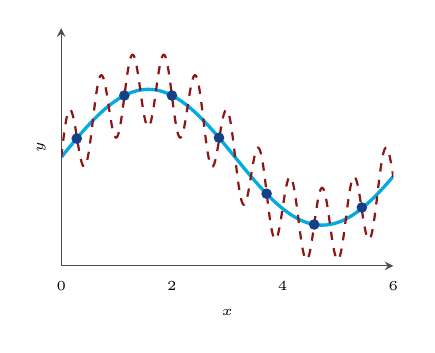
\begin{tikzpicture}[font=\scriptsize]
\begin{axis}[width=5.8cm, height=4.6cm,
	xlabel={$x$}, ylabel={$y$},
	xlabel style={font=\tiny}, ylabel style={font=\tiny},
	tick label style={font=\tiny}, axis lines=left,
	xmin=0, xmax=6, ymin=-1.6, ymax=1.9,
	axis line style={StanfordGray}, tick style={draw=none}, ytick=\empty]
	% la función razonable que efectivamente se obtiene
	\addplot[UCMBlue, very thick, domain=0:6, samples=100]{sin(deg(x))};
	% una alternativa igualmente compatible con los datos
	\addplot[StanfordRed, thick, dashed, domain=0:6, samples=400]
		{sin(deg(x)) + 0.55*sin(deg(11*x))};
	\addplot[only marks, mark=*, mark size=1.7pt, UCMNavy] coordinates {
		(0.28,0.276) (1.14,0.909) (2.00,0.909) (2.85,0.287)
		(3.71,-0.537) (4.57,-0.990) (5.43,-0.740)};
\end{axis}
\end{tikzpicture}
\end{center}
\vspace{-0.3em}
\fuente{Ambas curvas pasan por los mismos datos. Con capacidad de sobra, nada obliga al modelo a elegir la azul --- y aun as\'i la elige.}
\end{column}
\end{columns}
\vspace{0.2em}
\idea{Las regiones que \emph{s\'i} contienen datos restringen al resto a comportarse razonablemente. Por qu\'e ese contagio ocurre es, todav\'ia, una pregunta abierta.}
\end{frame}

%=====================================================================
\section{Factores que influyen en el ajuste}
%=====================================================================

\begin{frame}
\frametitle{¿Son los datos? El experimento de Zhang et al. (2017)}
\begin{columns}[c]
\begin{column}{6.5cm}
\begin{center}
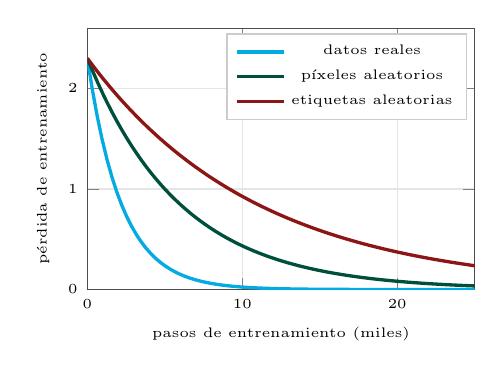
\begin{tikzpicture}
\begin{axis}[width=6.5cm, height=4.9cm,
	xlabel={pasos de entrenamiento (miles)}, ylabel={p\'erdida de entrenamiento},
	xlabel style={font=\tiny}, ylabel style={font=\tiny},
	tick label style={font=\tiny}, xmin=0, xmax=25, ymin=0, ymax=2.6,
	legend style={font=\tiny, at={(0.98,0.98)}, anchor=north east, draw=gray!40},
	grid=major, grid style={gray!20}, axis line style={StanfordGray}]
	\addplot[UCMBlue, very thick, domain=0:25, samples=80]{2.3*exp(-x/2.2)};
	\addplot[AccentGreen!60!black, very thick, domain=0:25, samples=80]{2.3*exp(-x/6.0)};
	\addplot[StanfordRed, very thick, domain=0:25, samples=80]{2.3*exp(-x/11.0)};
	\legend{datos reales, p\'ixeles aleatorios, etiquetas aleatorias}
\end{axis}
\end{tikzpicture}
\end{center}
\vspace{-0.4em}
\fuente{AlexNet sobre CIFAR-10 (50.000 im\'agenes, 10 clases) con SGD. Adaptado de Zhang et al.\ (2017a), fig.~20.1 de Prince.}
\end{column}
\begin{column}{5.7cm}
\begin{itemize}
	\item \textbf{Hip\'otesis:} ajustar es f\'acil porque las funciones del mundo real son ``simples''.
	\item \textbf{Prueba:} destruyamos toda estructura. (i) Reemplazar cada imagen por ruido gaussiano. (ii) Permutar las etiquetas al azar.
	\item \textbf{Resultado:} la red \textbf{sigue ajustando} el conjunto, solo que m\'as lento.
\end{itemize}
\vspace{0.4em}
\begin{exampleblock}{Conclusión incómoda}
\footnotesize
Las propiedades del conjunto de datos \textbf{no son} lo que hace f\'acil el ajuste. La red memoriza igual de bien un mapeo sin ninguna estructura.
\end{exampleblock}
\end{column}
\end{columns}
\end{frame}

\begin{frame}
\frametitle{¿Es la regularización? ¿Es el ruido de SGD?}
\footnotesize % ajuste de densidad
\begin{columns}[c]
\begin{column}{6.2cm}
\begin{center}
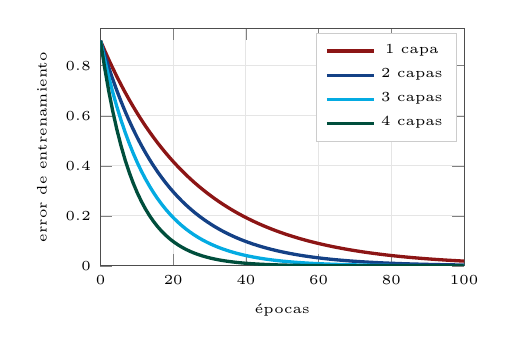
\begin{tikzpicture}
\begin{axis}[width=6.2cm, height=4.6cm,
	xlabel={\'epocas}, ylabel={error de entrenamiento},
	xlabel style={font=\tiny}, ylabel style={font=\tiny},
	tick label style={font=\tiny}, xmin=0, xmax=100, ymin=0, ymax=0.95,
	legend style={font=\tiny, at={(0.98,0.98)}, anchor=north east, draw=gray!40},
	grid=major, grid style={gray!20}, axis line style={StanfordGray}]
	\addplot[StanfordRed, very thick, domain=0:100, samples=90]{0.9*exp(-x/26)};
	\addplot[UCMNavy, very thick, domain=0:100, samples=90]{0.9*exp(-x/18)};
	\addplot[UCMBlue, very thick, domain=0:100, samples=90]{0.9*exp(-x/13)};
	\addplot[AccentGreen!60!black, very thick, domain=0:100, samples=90]{0.9*exp(-x/9)};
	\legend{1 capa, 2 capas, 3 capas, 4 capas}
\end{axis}
\end{tikzpicture}
\end{center}
\vspace{-0.4em}
\fuente{4.000 ejemplos MNIST-1D con \textbf{etiquetas aleatorias}, gradiente de lote completo, inicializaci\'on He, sin momento ni regularizaci\'on, $\eta=0{,}0025$. Los cuatro modelos tienen $\sim$15.200 par\'ametros. Fig.~20.2 de Prince.}
\end{column}
\begin{column}{5.9cm}
\begin{block}{Regularización}
\footnotesize
Zhang et al.\ mostraron que \textbf{ni $L_2$ (weight decay) ni Dropout} hacen falta para ajustar datos aleatorios. Queda la regularizaci\'on \emph{impl\'icita} del paso finito, pero esta crece con $\eta$ --- y ajustar no se vuelve m\'as f\'acil con $\eta$ grande.
\end{block}
\begin{block}{Estocasticidad}
\footnotesize
Keskar et al.\ (2017) ajustan bien con lotes de 5.000--6.000 im\'agenes, eliminando casi toda la aleatoriedad. La figura usa lote \textbf{completo}: proceso determinista, sin regularizaci\'on, etiquetas sin estructura, y el error igual llega a cero.
\end{block}
\end{column}
\end{columns}
\vspace{0.2em}
\idea{Esto sugiere que estas funciones de p\'erdida \textbf{quiz\'as no tengan m\'inimos locales} en absoluto. Ojo: no lo demuestra --- ver \emph{Problema 20.3}.}
\end{frame}

\begin{frame}
\frametitle{Sobreparametrización}
\footnotesize % ajuste de densidad
\begin{columns}[T]
\begin{column}{6.4cm}
\begin{itemize}
	\item Sobreparametrizar implica una \textbf{familia enorme de soluciones degeneradas}: casi siempre existe \emph{alguna} direcci\'on en la que mover los par\'ametros reduce la p\'erdida.
	\item En la pr\'actica las redes est\'an sobreparametrizadas por \textbf{uno o dos \'ordenes de magnitud}.
	\item Resultados te\'oricos: si la red es lo bastante ancha, SGD converge al m\'inimo global (Du et al., 2019a,b; Allen-Zhu et al., 2019; Zou et al., 2020).
	\item \textbf{Pero} las hip\'otesis son irreales: Du et al.\ exigen ancho $\Omega[I^{4}K^{2}]$ ($I$ datos, $K$ capas); Nguyen \& Hein suponen ancho mayor que el tama\~no del conjunto.
\end{itemize}
\end{column}
\begin{column}{5.8cm}
\begin{tcolorbox}[colback=UCMBlue!8, colframe=UCMBlue, arc=4pt, fontupper=\small]
\RaggedRight
``\emph{{\ldots}la degeneraci\'on de las soluciones cambia la naturaleza del problema: de buscar una aguja en un pajar, a buscar \textbf{un pajar de agujas}.}''
\vspace{0.2em}

\hfill --- Sejnowski (2020)
\end{tcolorbox}
\vspace{0.4em}
\begin{center}
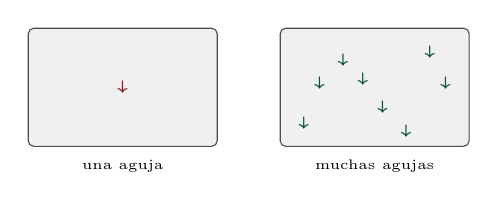
\begin{tikzpicture}[font=\tiny]
	\draw[draw=StanfordGray, fill=LightGray, rounded corners=2pt] (0,0) rectangle (2.4,1.5);
	\node[StanfordRed] at (1.2,0.75) {$\bm\downarrow$};
	\node[font=\tiny, anchor=north] at (1.2,-0.05) {una aguja};
	\draw[draw=StanfordGray, fill=LightGray, rounded corners=2pt] (3.2,0) rectangle (5.6,1.5);
	\foreach \x/\y in {0.3/0.3, 0.8/1.1, 1.3/0.5, 1.9/1.2, 0.5/0.8, 1.6/0.2, 2.1/0.8, 1.05/0.85}
		{\node[AccentGreen!60!black] at (3.2+\x,\y) {$\bm\downarrow$};}
	\node[font=\tiny, anchor=north] at (4.4,-0.05) {muchas agujas};
\end{tikzpicture}
\end{center}
\end{column}
\end{columns}
\vspace{0.2em}
\idea{La sobreparametrizaci\'on es, casi con certeza, el factor m\'as importante para que el ajuste sea f\'acil. Pero la teor\'ia todav\'ia \textbf{no explica} el desempe\~no emp\'irico.}
\end{frame}

\begin{frame}
\frametitle{Activación, inicialización y profundidad}
\scriptsize % ajuste de densidad
\begin{columns}[T]
\begin{column}{6.1cm}
\begin{block}{Función de activación (sí importa)}
Si la activaci\'on solo var\'ia en una porci\'on peque\~na del rango de entrada, la red es \textbf{m\'as dif\'icil de ajustar}. Sigmoide y tanh tienen colas planas: donde la activaci\'on es casi constante el gradiente es casi nulo y el mecanismo de mejora desaparece. ReLU var\'ia en medio rango; Leaky ReLU, en todo.
\end{block}
\begin{block}{Inicialización (importa poco)}
Xavier/He son necesarias para evitar gradientes explosivos o evanescentes en redes profundas. Pero Liu et al.\ (2023c) muestran que multiplicar la varianza de He solo hace falta \textbf{m\'as iteraciones}: no impide el ajuste. Refleja la distancia extra que deben recorrer los pesos.
\end{block}
\end{column}
\begin{column}{6.1cm}
\begin{alertblock}{Profundidad: la hipótesis del billete de lotería}
Frankle \& Carbin (2019): (i) entrenar la red, (ii) podar los pesos de menor magnitud, (iii) \textbf{reentrenar desde los mismos pesos iniciales}. El resultado iguala o supera al original.
\vspace{0.3em}

Si en cambio se reinicializan los pesos al azar, \textbf{no funciona}.
\vspace{0.3em}

$\Rightarrow$ la red sobreparametrizada conten\'ia \textbf{subredes entrenables} suficientes por s\'i solas: los \emph{billetes ganadores}.
\end{alertblock}
\vspace{0.2em}
No hay evidencia definitiva de que la p\'erdida sea m\'as o menos convexa al aumentar la profundidad: los problemas de gradientes explosivos, evanescentes o \emph{astillados} son (discutiblemente) num\'ericos.
\end{column}
\end{columns}
\vspace{0.2em}
\idea{Quiz\'a lo que var\'ia con la profundidad, a igual n\'umero de par\'ametros, es el \textbf{n\'umero efectivo de subredes} disponibles. La caracterizaci\'on precisa de esa idea todav\'ia no existe.}
\end{frame}

\begin{frame}
\frametitle{Balance: qué importa para ajustar y qué no}
\begin{center}
\footnotesize
\begin{tabular}{llp{6.1cm}}
\toprule
\textbf{Factor} & \textbf{¿Importa?} & \textbf{Evidencia}\\
\midrule
Sobreparametrizaci\'on & \textcolor{AccentGreen!60!black}{\textbf{S\'i}}
	& Familia degenerada de soluciones; garant\'ias de convergencia si el ancho es suficiente\\
Funci\'on de activaci\'on & \textcolor{AccentGreen!60!black}{\textbf{S\'i}}
	& Colas planas $\Rightarrow$ gradiente nulo; ReLU $>$ sigmoide\\[3pt]
Estructura de los datos & \textcolor{StanfordRed}{\textbf{No}}
	& Se ajustan p\'ixeles y etiquetas aleatorias (Zhang et al., 2017a)\\
Regularizaci\'on & \textcolor{StanfordRed}{\textbf{No}}
	& Sin $L_2$ ni Dropout el ajuste igual llega a cero\\
Aleatoriedad de SGD & \textcolor{StanfordRed}{\textbf{No}}
	& Lote completo determinista tambi\'en ajusta\\
Inicializaci\'on & \textcolor{StanfordGray}{\textbf{Poco}}
	& Cambia la velocidad, no el resultado (salvo gradientes ines\-ta\-bles)\\
Profundidad & \textcolor{StanfordGray}{\textbf{Poco claro}}
	& Redes profundas ajustan en menos \'epocas, pero puede ser un artefacto de la inicializaci\'on\\
\bottomrule
\end{tabular}
\end{center}
\vspace{0.5em}
\idea{El resultado m\'as inc\'omodo del cap\'itulo: casi todo lo que ense\~namos como ``buenas pr\'acticas'' de entrenamiento afecta \textbf{la generalizaci\'on}, no la capacidad de ajustar. Son dos preguntas distintas.}
\end{frame}

%=====================================================================
\section{Propiedades de la función de pérdida}
%=====================================================================

\begin{frame}
\frametitle{Muchos mínimos globales (y por construcción)}
\begin{columns}[T]
\begin{column}{6.2cm}
Cuatro fuentes de \textbf{soluciones equivalentes} que producen exactamente la misma salida:
\begin{itemize}
	\item \textbf{Permutaci\'on}: reordenar las unidades ocultas de una capa (con sus pesos) no cambia nada.
	\item \textbf{Canales}: en una CNN, permutar canales y n\'ucleos de convoluci\'on.
	\item \textbf{Escalado de ReLU}: multiplicar el peso \emph{antes} de un ReLU por $\alpha>0$ y dividir el de \emph{despu\'es} por $\alpha$.
	\item \textbf{BatchNorm}: reinicia media y varianza de cada unidad, generando otro conjunto de redundancias.
\end{itemize}
\end{column}
\begin{column}{6.0cm}
\begin{center}
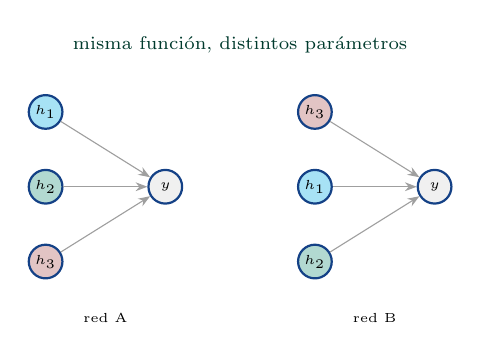
\begin{tikzpicture}[font=\tiny, scale=0.95, transform shape,
	nn/.style={circle, draw=UCMNavy, thick, minimum size=4.5mm, inner sep=0pt}]
	% red A
	\begin{scope}
		\node[nn, fill=UCMBlue!35] (a1) at (0,1.0) {$h_1$};
		\node[nn, fill=AccentGreen!30] (a2) at (0,0.0) {$h_2$};
		\node[nn, fill=StanfordRed!25] (a3) at (0,-1.0) {$h_3$};
		\node[nn, fill=LightGray] (ao) at (1.6,0) {$y$};
		\foreach \i in {1,2,3}{\draw[-{Stealth[length=1.5mm]}, gray!75] (a\i) -- (ao);}
		\node at (0.8,-1.75) {red A};
	\end{scope}
	% red B
	\begin{scope}[xshift=3.6cm]
		\node[nn, fill=StanfordRed!25] (b1) at (0,1.0) {$h_3$};
		\node[nn, fill=UCMBlue!35] (b2) at (0,0.0) {$h_1$};
		\node[nn, fill=AccentGreen!30] (b3) at (0,-1.0) {$h_2$};
		\node[nn, fill=LightGray] (bo) at (1.6,0) {$y$};
		\foreach \i in {1,2,3}{\draw[-{Stealth[length=1.5mm]}, gray!75] (b\i) -- (bo);}
		\node at (0.8,-1.75) {red B};
	\end{scope}
	\node[font=\scriptsize, text=AccentGreen!45!black] at (2.6,1.9)
		{misma funci\'on, distintos par\'ametros};
\end{tikzpicture}
\end{center}
\vspace{0.3em}
\footnotesize
Adem\'as, el m\'inimo global solo depende de la salida \textbf{en los datos de entrenamiento}. En redes sobreparametrizadas hay familias que coinciden en los datos y \textbf{difieren entre ellos}: todas son m\'inimos globales.
\end{column}
\end{columns}
\end{frame}

\begin{frame}
\frametitle{La ruta hacia el mínimo}
\footnotesize % ajuste de densidad
\begin{columns}[c]
\begin{column}{6.2cm}
\begin{center}
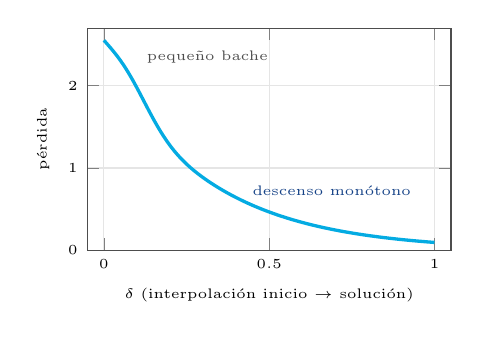
\begin{tikzpicture}
\begin{axis}[width=6.2cm, height=4.4cm,
	xlabel={$\delta$ (interpolaci\'on inicio $\to$ soluci\'on)}, ylabel={p\'erdida},
	xlabel style={font=\tiny}, ylabel style={font=\tiny},
	tick label style={font=\tiny}, xmin=-0.05, xmax=1.05, ymin=0, ymax=2.7,
	xtick={0,0.5,1}, axis line style={StanfordGray},
	grid=major, grid style={gray!20}]
	\addplot[UCMBlue, very thick, domain=0:1, samples=100]
		{2.3*exp(-3.2*x) + 0.35*exp(-90*(x-0.06)^2)};
	\node[font=\tiny, text=StanfordGray, anchor=west] at (axis cs:0.10,2.35) {peque\~no bache};
	\node[font=\tiny, text=UCMNavy, anchor=south west] at (axis cs:0.42,0.55)
		{descenso mon\'otono};
\end{axis}
\end{tikzpicture}
\end{center}
\vspace{-0.4em}
\fuente{Corte lineal entre los par\'ametros iniciales ($\delta{=}0$) y los entrenados ($\delta{=}1$). Goodfellow et al.\ (2015b); fig.~20.5a de Prince.}
\end{column}
\begin{column}{6.0cm}
\begin{itemize}
	\item En \textbf{l\'inea recta} desde la inicializaci\'on hasta la soluci\'on la p\'erdida baja de forma casi mon\'otona, en muchas arquitecturas y activaciones.
	\item Las trayectorias reales no son rectas, pero \textbf{viven en subespacios de baja dimensi\'on} (Li et al., 2018b): grandes regiones casi convexas capturan la trayectoria y la encauzan.
	\item Li et al.\ (2018a): restringiendo la optimizaci\'on a un subespacio \textbf{aleatorio} de 750 dimensiones ($0{,}4\%$ de los par\'ametros) se alcanza el 90\,\% del rendimiento. Lo llaman \textbf{dimensi\'on intr\'inseca}.
\end{itemize}
\end{column}
\end{columns}
\vspace{0.2em}
\idea{El problema de optimizaci\'on tiene millones de dimensiones, pero el \textbf{camino recorrido} es de dimensi\'on baj\'isima. Ah\'i puede estar buena parte de la explicaci\'on.}
\end{frame}

\begin{frame}
\frametitle{Conexiones entre mínimos}
\footnotesize % ajuste de densidad
\begin{columns}[c]
\begin{column}{6.3cm}
\begin{center}
\scalebox{0.70}{%
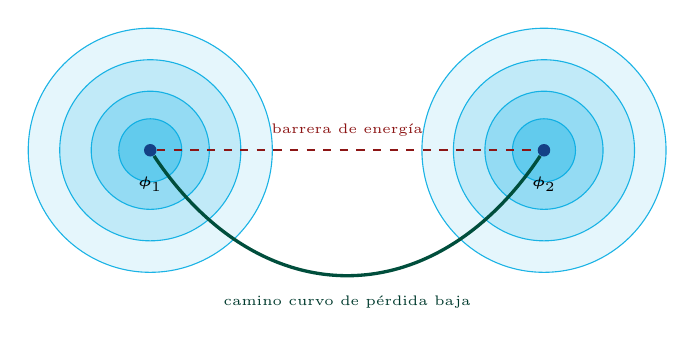
\begin{tikzpicture}[font=\scriptsize]
	% contornos del paisaje
	\begin{scope}
		\foreach \r/\op in {1.55/0.10, 1.15/0.16, 0.75/0.24, 0.40/0.34}{
			\draw[UCMBlue, opacity=0.9, fill=UCMBlue, fill opacity=\op]
				(0,0) circle (\r);
			\draw[UCMBlue, opacity=0.9, fill=UCMBlue, fill opacity=\op]
				(5.0,0) circle (\r);
		}
	\end{scope}
	\node[circle, fill=UCMNavy, inner sep=1.6pt] (m1) at (0,0) {};
	\node[circle, fill=UCMNavy, inner sep=1.6pt] (m2) at (5.0,0) {};
	\node[font=\tiny, anchor=north] at (0,-0.22) {$\bm\phi_1$};
	\node[font=\tiny, anchor=north] at (5.0,-0.22) {$\bm\phi_2$};

	% barrera lineal
	\draw[StanfordRed, thick, dashed] (m1) -- (m2);
	\node[font=\tiny, text=StanfordRed, anchor=south] at (2.5,0.06) {barrera de energ\'ia};

	% camino curvo de baja pérdida
	\draw[AccentGreen!60!black, very thick]
		(m1) .. controls (1.4,-2.1) and (3.6,-2.1) .. (m2);
	\node[font=\tiny, text=AccentGreen!45!black, anchor=north] at (2.5,-1.72)
		{camino curvo de p\'erdida baja};
\end{tikzpicture}}
\end{center}
\vspace{-0.2em}
\fuente{Corte de la p\'erdida de DenseNet sobre CIFAR-10. Draxler et al.\ (2018); fig.~20.7 de Prince.}
\end{column}
\begin{column}{5.9cm}
\begin{itemize}
	\item Entre dos m\'inimos hallados \emph{independientemente} la p\'erdida \textbf{sube} si se interpola en l\'inea recta: no est\'an linealmente conectados.
	\item Frankle et al.\ (2020): esa barrera \textbf{desaparece} si ambas redes se entrenan id\'enticamente al principio y solo despu\'es divergen. La soluci\'on queda determinada \textbf{temprano}.
	\item Draxler et al.\ (2018): siempre es posible construir un \textbf{camino curvo} donde la p\'erdida se mantiene baja. Cuanto m\'as ancha y profunda la red, m\'as f\'acil.
\end{itemize}
\vspace{0.3em}
\begin{exampleblock}{Conclusión}
\footnotesize
No hay ``valles aislados'': parece haber \textbf{una sola variedad conexa} de p\'erdida baja.
\end{exampleblock}
\end{column}
\end{columns}
\end{frame}

\begin{frame}
\frametitle{Curvatura}
\footnotesize % ajuste de densidad
\begin{columns}[c]
\begin{column}{6.1cm}
\begin{center}
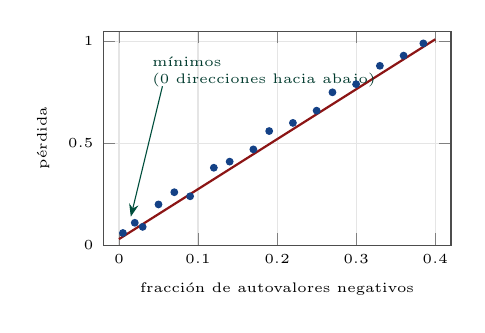
\begin{tikzpicture}
\begin{axis}[width=6.0cm, height=4.3cm,
	xlabel={fracci\'on de autovalores negativos}, ylabel={p\'erdida},
	xlabel style={font=\tiny}, ylabel style={font=\tiny},
	tick label style={font=\tiny}, xmin=-0.02, xmax=0.42, ymin=0, ymax=1.05,
	axis line style={StanfordGray}, grid=major, grid style={gray!20}]
	\addplot[only marks, mark=*, mark size=1.2pt, UCMNavy] coordinates {
		(0.005,0.06) (0.02,0.11) (0.03,0.09) (0.05,0.20) (0.07,0.26)
		(0.09,0.24) (0.12,0.38) (0.14,0.41) (0.17,0.47) (0.19,0.56)
		(0.22,0.60) (0.25,0.66) (0.27,0.75) (0.30,0.79) (0.33,0.88)
		(0.36,0.93) (0.385,0.99)};
	\addplot[StanfordRed, thick, domain=0:0.40, samples=2]{2.45*x+0.03};
	\node[font=\tiny, text=AccentGreen!45!black, anchor=west, align=left]
		at (axis cs:0.03,0.85) {m\'inimos\\ (0 direcciones hacia abajo)};
	\draw[AccentGreen!60!black, -{Stealth[length=1.6mm]}]
		(axis cs:0.055,0.78) -- (axis cs:0.015,0.14);
\end{axis}
\end{tikzpicture}
\end{center}
\vspace{-0.4em}
\fuente{Dauphin et al.\ (2014); fig.~20.8 de Prince.}
\end{column}
\begin{column}{6.0cm}
\begin{itemize}
	\item En puntos con gradiente cero, la proporci\'on de direcciones que \textbf{bajan} disminuye a medida que baja la p\'erdida.
	\item Es decir: los puntos cr\'iticos con p\'erdida alta son \textbf{puntos silla}, no m\'inimos. Los verdaderos m\'inimos aparecen todos con p\'erdida baja.
	\item Baldi \& Hornik (1989) ya lo hab\'ian probado en redes superficiales: solo puntos silla, ning\'un m\'inimo local.
\end{itemize}
\vspace{0.3em}
\begin{block}{Zona \emph{Goldilocks}}
\footnotesize
Fort \& Scherlis (2019): la curvatura de la superficie es \textbf{inusualmente positiva} cuando la norma $\ell_2$ de los pesos cae en cierto rango. Las inicializaciones de He y Xavier caen justo ah\'i.
\end{block}
\end{column}
\end{columns}
\vspace{0.2em}
\idea{No parece haber m\'inimos locales malos. La dificultad te\'orica (NP-dureza) es real \emph{en el peor caso}, pero las p\'erdidas que encontramos en la pr\'actica no son el peor caso.}
\end{frame}

%=====================================================================
\section{Factores que determinan la generalización}
%=====================================================================

\begin{frame}
\frametitle{El algoritmo elige a cuál mínimo llegar}
\footnotesize % ajuste de densidad
\begin{columns}[c]
\begin{column}{6.1cm}
\begin{center}
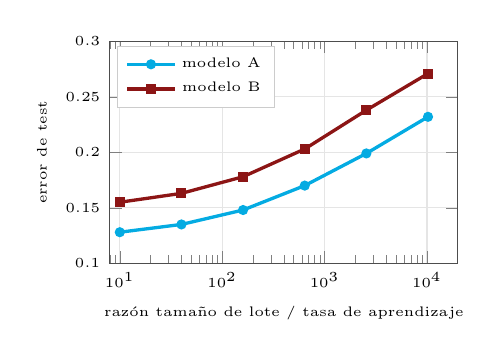
\begin{tikzpicture}
\begin{axis}[width=6.0cm, height=4.4cm,
	xlabel={raz\'on tama\~no de lote / tasa de aprendizaje},
	ylabel={error de test},
	xlabel style={font=\tiny}, ylabel style={font=\tiny},
	tick label style={font=\tiny}, xmode=log, xmin=8, xmax=20000,
	ymin=0.10, ymax=0.30, axis line style={StanfordGray},
	grid=major, grid style={gray!20},
	legend style={font=\tiny, at={(0.02,0.98)}, anchor=north west, draw=gray!40}]
	\addplot[UCMBlue, very thick, mark=*, mark size=1.2pt] coordinates {
		(10,0.128) (40,0.135) (160,0.148) (640,0.170) (2560,0.199) (10240,0.232)};
	\addplot[StanfordRed, very thick, mark=square*, mark size=1.2pt] coordinates {
		(10,0.155) (40,0.163) (160,0.178) (640,0.203) (2560,0.238) (10240,0.271)};
	\legend{modelo A, modelo B}
\end{axis}
\end{tikzpicture}
\end{center}
\vspace{-0.4em}
\fuente{CIFAR-10. Adaptado de He et al.\ (2019); fig.~20.10 de Prince.}
\end{column}
\begin{column}{6.0cm}
\begin{itemize}
	\item Como la red est\'a sobreparametrizada, es el \textbf{proceso de entrenamiento} el que decide a cu\'al de los m\'inimos degenerados se llega.
	\item SGD generaliza mejor que el gradiente de lote completo (LeCun et al., 2012).
	\item Lotes \textbf{peque\~nos} generalizan mejor cuando no hay otra regularizaci\'on (Keskar et al., 2017); tasas de aprendizaje \textbf{grandes} tambi\'en.
	\item Lo que importa es la \textbf{raz\'on} tama\~no de lote / tasa de aprendizaje (Jastrz\k{e}bski et al., 2018; He et al., 2019).
\end{itemize}
\end{column}
\end{columns}
\vspace{0.2em}
\idea{Todo esto es coherente con que SGD a\~nade una \textbf{regularizaci\'on impl\'icita} cuya magnitud depende de $\eta$: cambia la trayectoria y la lleva a una zona que generaliza bien.}
\end{frame}

\begin{frame}
\frametitle{Planitud del mínimo}
\footnotesize % ajuste de densidad
\begin{columns}[c]
\begin{column}{6.3cm}
\begin{center}
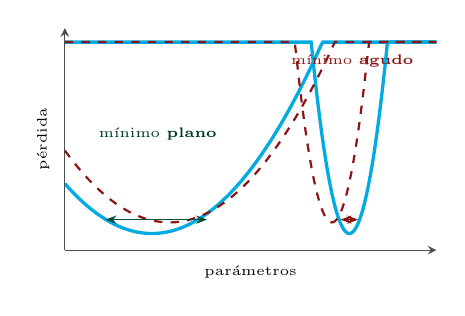
\begin{tikzpicture}
\begin{axis}[width=6.3cm, height=4.4cm,
	xlabel={par\'ametros}, ylabel={p\'erdida},
	xlabel style={font=\tiny}, ylabel style={font=\tiny},
	axis lines=left, xmin=-3.2, xmax=3.2, ymin=-0.1, ymax=1.5,
	xtick=\empty, ytick=\empty, axis line style={StanfordGray}]
	% pérdida de entrenamiento
	\addplot[UCMBlue, very thick, domain=-3.2:3.2, samples=250]
		{min(1.4, 0.10*(x+1.7)^2*1.6 + 0.02)};
	\addplot[UCMBlue, very thick, domain=-3.2:3.2, samples=250]
		{min(1.4, 3.2*(x-1.7)^2 + 0.02)};
	% pérdida de test, ligeramente desplazada
	\addplot[StanfordRed, thick, dashed, domain=-3.2:3.2, samples=250]
		{min(1.4, 0.10*(x+1.4)^2*1.6 + 0.10)};
	\addplot[StanfordRed, thick, dashed, domain=-3.2:3.2, samples=250]
		{min(1.4, 3.2*(x-1.4)^2 + 0.10)};
	\node[font=\tiny, text=AccentGreen!45!black, anchor=south] at (axis cs:-1.6,0.62)
		{m\'inimo \textbf{plano}};
	\node[font=\tiny, text=StanfordRed, anchor=south] at (axis cs:1.75,1.15)
		{m\'inimo \textbf{agudo}};
	\draw[AccentGreen!60!black, {Stealth[length=1.4mm]}-{Stealth[length=1.4mm]}]
		(axis cs:-2.5,0.12) -- (axis cs:-0.75,0.12);
	\draw[StanfordRed, {Stealth[length=1.4mm]}-{Stealth[length=1.4mm]}]
		(axis cs:1.55,0.12) -- (axis cs:1.85,0.12);
\end{axis}
\end{tikzpicture}
\end{center}
\vspace{-0.5em}
\fuente{Azul: p\'erdida de entrenamiento. Rojo punteado: p\'erdida de test, ligeramente desalineada. Keskar et al.\ (2017); fig.~20.11 de Prince.}
\end{column}
\begin{column}{5.9cm}
\begin{itemize}
	\item Idea (Hochreiter \& Schmidhuber, 1997): en un m\'inimo \textbf{plano}, un peque\~no error en los par\'ametros --- o un peque\~no desajuste entre la p\'erdida de train y la de test --- casi no cuesta.
	\item Longitud de descripci\'on m\'inima: en m\'inimos anchos se necesitan \textbf{menos bits} para almacenar los pesos $\Rightarrow$ deber\'ian generalizar mejor.
	\item Promediar pesos a lo largo de la trayectoria (Izmailov et al., 2018) aplana la superficie \textbf{y} mejora la generalizaci\'on.
\end{itemize}
\end{column}
\end{columns}
\vspace{0.2em}
\idea{Con cautela: la planitud medida puede alterarse con \textbf{reparametrizaciones triviales} de ReLU (Dinh et al., 2017), y al aleatorizar etiquetas en CIFAR el m\'inimo \emph{no} se vuelve m\'as agudo pese a que generalizar es imposible (Neyshabur et al., 2017).}
\end{frame}

\begin{frame}
\frametitle{Arquitectura: el sesgo inductivo}
\begin{columns}[T]
\begin{column}{6.2cm}
\begin{itemize}
	\item El \textbf{sesgo inductivo} de una red lo fija su arquitectura, y elegirla bien mejora dr\'asticamente la generalizaci\'on.
	\item Las \textbf{CNN} suponen que las estad\'isticas de la entrada son iguales en todas las posiciones, y por eso comparten par\'ametros a lo largo del espacio.
	\item Los \textbf{transformers} se ajustan a datos invariantes a permutaciones.
	\item Las \textbf{GNN} se ajustan a datos sobre grafos irregulares.
\end{itemize}
\vspace{0.3em}
\footnotesize
Emparejar la arquitectura con las propiedades de los datos generaliza mejor que una red totalmente conectada gen\'erica.
\end{column}
\begin{column}{5.9cm}
\begin{center}
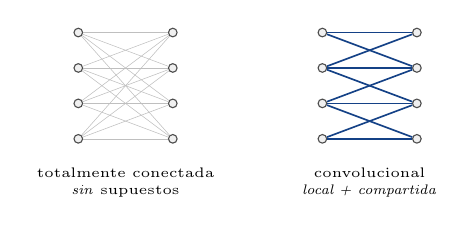
\begin{tikzpicture}[font=\tiny,
	cap/.style={rectangle, draw=UCMNavy, thick, minimum width=0.55cm,
		minimum height=1.5cm, fill=UCMBlue!20}]
	% totalmente conectada: todas las conexiones
	\begin{scope}
		\foreach \i/\y in {0/0, 1/0.45, 2/0.9, 3/1.35}{
			\node[circle,draw=StanfordGray,fill=LightGray,inner sep=1.1pt] (u\i) at (0,\y) {};
			\node[circle,draw=StanfordGray,fill=LightGray,inner sep=1.1pt] (v\i) at (1.2,\y) {};}
		\foreach \a in {0,...,3}\foreach \b in {0,...,3}
			{\draw[gray!50, very thin] (u\a) -- (v\b);}
		\node[anchor=north, align=center] at (0.6,-0.25)
			{totalmente conectada\\ \emph{sin} supuestos};
	\end{scope}
	% convolucional: conexiones locales compartidas
	\begin{scope}[xshift=3.1cm]
		\foreach \i/\y in {0/0, 1/0.45, 2/0.9, 3/1.35}{
			\node[circle,draw=StanfordGray,fill=LightGray,inner sep=1.1pt] (p\i) at (0,\y) {};
			\node[circle,draw=StanfordGray,fill=LightGray,inner sep=1.1pt] (q\i) at (1.2,\y) {};}
		\foreach \a/\b in {0/0, 0/1, 1/0, 1/1, 1/2, 2/1, 2/2, 2/3, 3/2, 3/3}
			{\draw[UCMNavy, semithick] (p\a) -- (q\b);}
		\node[anchor=north, align=center] at (0.6,-0.25)
			{convolucional\\ \emph{local + compartida}};
	\end{scope}
\end{tikzpicture}
\end{center}
\vspace{0.6em}
\begin{exampleblock}{Lectura}
\footnotesize
Restringir lo que la red \emph{puede} representar no es una limitaci\'on: es informaci\'on que le damos gratis sobre el problema.
\end{exampleblock}
\end{column}
\end{columns}
\end{frame}

\begin{frame}
\frametitle{La norma de los pesos y el \emph{grokking} \footnote{\url{https://arxiv.org/abs/2201.02177}}}
\footnotesize % ajuste de densidad
\begin{columns}[c]
\begin{column}{6.2cm}
\begin{center}
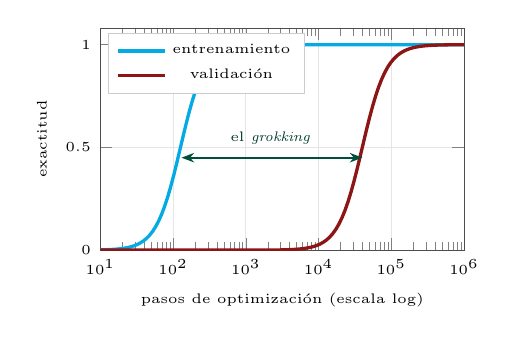
\begin{tikzpicture}
\begin{axis}[width=6.2cm, height=4.4cm,
	xlabel={pasos de optimizaci\'on (escala log)}, ylabel={exactitud},
	xlabel style={font=\tiny}, ylabel style={font=\tiny},
	tick label style={font=\tiny}, xmode=log, xmin=10, xmax=1000000,
	ymin=0, ymax=1.08, axis line style={StanfordGray},
	grid=major, grid style={gray!20},
	legend style={font=\tiny, at={(0.02,0.98)}, anchor=north west, draw=gray!40}]
	\addplot[UCMBlue, very thick, domain=1:6, samples=120]
		({10^x},{1/(1+exp(-6*(x-2.1)))});
	\addplot[StanfordRed, very thick, domain=1:6, samples=120]
		({10^x},{1/(1+exp(-6*(x-4.6)))});
	\legend{entrenamiento, validaci\'on}
	\draw[AccentGreen!60!black, {Stealth[length=1.6mm]}-{Stealth[length=1.6mm]}, thick]
		(axis cs:130,0.45) -- (axis cs:40000,0.45);
	\node[font=\tiny, text=AccentGreen!45!black, anchor=south] at (axis cs:2200,0.47)
		{el \emph{grokking}};
\end{axis}
\end{tikzpicture}
\end{center}
\vspace{-0.4em}
\fuente{Power et al.\ (2022); Liu et al.\ (2023c); fig.~20.13 de Prince.}
\end{column}
\begin{column}{5.9cm}
\begin{itemize}
	\item La norma $\ell_2$ de los pesos se relaciona (indirectamente) con la \textbf{constante de Lipschitz} del modelo.
	\item \textbf{Muy peque\~na}: el modelo no puede cambiar lo bastante r\'apido para capturar la funci\'on.
	\item \textbf{Muy grande}: var\'ia demasiado entre los datos y no interpola con suavidad.
	\item Entre medio est\'a la \textbf{zona Goldilocks}, donde tambi\'en generaliza bien (Fort \& Scherlis, 2019).
\end{itemize}
\vspace{0.3em}
\begin{exampleblock}{Explicación del \emph{grokking}}
\footnotesize
Si la norma inicial es demasiado grande, el modelo \textbf{ajusta} pronto pero var\'ia mucho entre los datos. La regularizaci\'on va bajando la norma; al entrar en la zona Goldilocks la generalizaci\'on mejora \textbf{de golpe}, miles de \'epocas despu\'es.
\end{exampleblock}
\end{column}
\end{columns}
\end{frame}

\begin{frame}
\frametitle{Sobreparametrización y doble descenso}
\footnotesize % ajuste de densidad
\begin{columns}[c]
\begin{column}{6.6cm}
\begin{center}
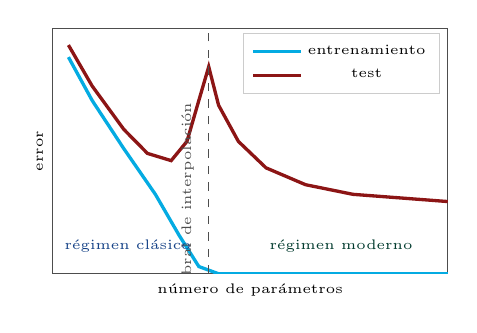
\begin{tikzpicture}
\begin{axis}[width=6.6cm, height=4.7cm,
	xlabel={n\'umero de par\'ametros}, ylabel={error},
	xlabel style={font=\tiny}, ylabel style={font=\tiny},
	tick label style={font=\tiny}, xmin=0, xmax=10, ymin=0, ymax=1.02,
	xtick=\empty, ytick=\empty, axis line style={StanfordGray},
	legend style={font=\tiny, at={(0.98,0.98)}, anchor=north east, draw=gray!40}]
	% error de entrenamiento
	\addplot[UCMBlue, very thick] coordinates {
		(0.4,0.90) (1.0,0.72) (1.8,0.52) (2.6,0.33) (3.2,0.16) (3.7,0.03)
		(4.2,0.0) (5,0.0) (7,0.0) (10,0.0)};
	% error de test: doble descenso
	\addplot[StanfordRed, very thick] coordinates {
		(0.4,0.95) (1.0,0.78) (1.8,0.60) (2.4,0.50) (3.0,0.47) (3.4,0.55)
		(3.7,0.72) (3.95,0.86) (4.2,0.70) (4.7,0.55) (5.4,0.44)
		(6.4,0.37) (7.6,0.33) (10,0.30)};
	\legend{entrenamiento, test}
	\draw[StanfordGray, dashed] (axis cs:3.95,0) -- (axis cs:3.95,1.02);
	\node[font=\tiny, text=StanfordGray, anchor=south, rotate=90]
		at (axis cs:3.82,0.30) {umbral de interpolaci\'on};
	\node[font=\tiny, text=UCMNavy, anchor=south] at (axis cs:1.9,0.05)
		{r\'egimen cl\'asico};
	\node[font=\tiny, text=AccentGreen!45!black, anchor=south] at (axis cs:7.3,0.05)
		{r\'egimen moderno};
\end{axis}
\end{tikzpicture}
\end{center}
\end{column}
\begin{column}{5.6cm}
\begin{itemize}
	\item El compromiso sesgo/varianza cl\'asico dice que pasado cierto punto el error de test debe \textbf{subir}.
	\item Y sube --- hasta el \textbf{umbral de interpolaci\'on}, donde hay tantos par\'ametros como datos. Despu\'es \textbf{vuelve a bajar}.
	\item Explicaci\'on propuesta: sobreparametrizada, la red tiene m\'as libertad para ser \textbf{suave} entre los datos.
	\item En t\'erminos de la norma: cerca del umbral el modelo se \emph{contorsiona} para pasar por todos los puntos y su norma crece; con m\'as anchura, la varianza de He/Glorot ($\propto 1/\text{ancho}$) hace que los pesos casi no necesiten moverse.
\end{itemize}
\end{column}
\end{columns}
\vspace{0.2em}
\idea{La curva en U de la teor\'ia cl\'asica no est\'a mal: est\'a \textbf{incompleta}. Es solo la mitad izquierda del dibujo.}
\end{frame}

\begin{frame}
\frametitle{Salir de la variedad de datos: ejemplos adversarios}
\footnotesize % ajuste de densidad
\begin{center}
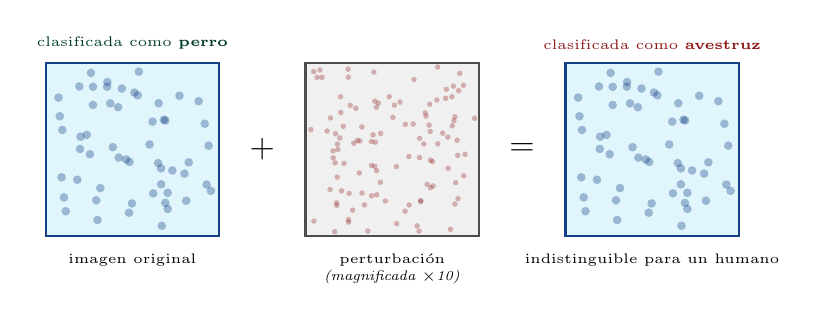
\begin{tikzpicture}[font=\scriptsize]
	% imagen original
	\begin{scope}
		\draw[draw=UCMNavy, thick, fill=UCMBlue!12] (0,0) rectangle (2.2,2.2);
		\pgfmathsetseed{2024}
		\foreach \i in {1,...,55}{\fill[UCMNavy, opacity=0.35]
			({0.1+random()*2.0},{0.1+random()*2.0}) circle (0.055);}
		\node[anchor=north, font=\tiny] at (1.1,-0.1) {imagen original};
		\node[anchor=south, font=\tiny, text=AccentGreen!45!black] at (1.1,2.25)
			{clasificada como \textbf{perro}};
	\end{scope}
	\node[font=\large] at (2.75,1.1) {$+$};
	% perturbación
	\begin{scope}[xshift=3.3cm]
		\draw[draw=StanfordGray, thick, fill=LightGray] (0,0) rectangle (2.2,2.2);
		\foreach \i in {1,...,110}{\fill[StanfordRed, opacity=0.30]
			({0.05+random()*2.1},{0.05+random()*2.1}) circle (0.035);}
		\node[anchor=north, font=\tiny, align=center] at (1.1,-0.1)
			{perturbaci\'on\\ \emph{(magnificada $\times$10)}};
	\end{scope}
	\node[font=\large] at (6.05,1.1) {$=$};
	% imagen adversaria
	\begin{scope}[xshift=6.6cm]
		\draw[draw=UCMNavy, thick, fill=UCMBlue!12] (0,0) rectangle (2.2,2.2);
		\pgfmathsetseed{2024}
		\foreach \i in {1,...,55}{\fill[UCMNavy, opacity=0.35]
			({0.1+random()*2.0},{0.1+random()*2.0}) circle (0.055);}
		\node[anchor=north, font=\tiny] at (1.1,-0.1) {indistinguible para un humano};
		\node[anchor=south, font=\tiny, text=StanfordRed] at (1.1,2.25)
			{clasificada como \textbf{avestruz}};
	\end{scope}
\end{tikzpicture}
\end{center}
\vspace{0.3em}
\begin{columns}[T]
\begin{column}{6.1cm}
\begin{itemize}
	\item Se perturba una imagen bien clasificada siguiendo el \textbf{gradiente de la salida respecto de la entrada}, hasta que la clase cambia.
	\item Uno esperar\'ia algo a medio camino entre perro y avestruz. En la pr\'actica la imagen se ve \textbf{igual}.
\end{itemize}
\end{column}
\begin{column}{6.1cm}
\begin{itemize}
	\item Hay posiciones \textbf{cercanas pero no sobre} la variedad de datos que se clasifican mal.
	\item Mejor explicaci\'on actual (Ilyas et al., 2019): no es falta de robustez fuera de la distribuci\'on; el ataque \textbf{explota se\~nales reales} de la distribuci\'on de entrenamiento, de norma peque\~na e imperceptibles para nosotros.
\end{itemize}
\end{column}
\end{columns}
\vspace{0.2em}
\fuente{Szegedy et al.\ (2014); Goodfellow et al.\ (2015a); fig.~20.14 de Prince. Adem\'as, D'Amour et al.\ (2020) muestran que modelos id\'enticos con distinta semilla var\'ian enormemente sobre datos corrompidos.}
\end{frame}

%=====================================================================
\section{¿Hacen falta tantos parámetros?}
%=====================================================================

\begin{frame}
\frametitle{Poda (\emph{pruning})}
\begin{columns}[c]
\begin{column}{6.0cm}
\begin{center}
\scalebox{0.82}{%
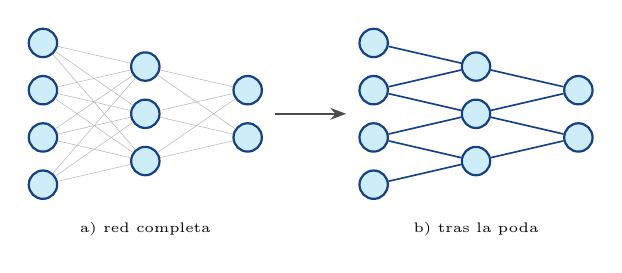
\begin{tikzpicture}[font=\tiny,
	nn/.style={circle, draw=UCMNavy, thick, fill=UCMBlue!20, minimum size=3.6mm, inner sep=0pt}]
	% red completa
	\begin{scope}
		\foreach \i/\y in {0/0, 1/0.6, 2/1.2, 3/1.8}{\node[nn] (a\i) at (0,\y) {};}
		\foreach \i/\y in {0/0.3, 1/0.9, 2/1.5}{\node[nn] (b\i) at (1.3,\y) {};}
		\foreach \i/\y in {0/0.6, 1/1.2}{\node[nn] (c\i) at (2.6,\y) {};}
		\foreach \p in {0,...,3}\foreach \q in {0,1,2}
			{\draw[gray!55, very thin] (a\p) -- (b\q);}
		\foreach \p in {0,1,2}\foreach \q in {0,1}
			{\draw[gray!55, very thin] (b\p) -- (c\q);}
		\node[anchor=north] at (1.3,-0.35) {a) red completa};
	\end{scope}
	% red podada
	\begin{scope}[xshift=4.2cm]
		\foreach \i/\y in {0/0, 1/0.6, 2/1.2, 3/1.8}{\node[nn] (d\i) at (0,\y) {};}
		\foreach \i/\y in {0/0.3, 1/0.9, 2/1.5}{\node[nn] (e\i) at (1.3,\y) {};}
		\foreach \i/\y in {0/0.6, 1/1.2}{\node[nn] (f\i) at (2.6,\y) {};}
		\foreach \p/\q in {0/0, 1/0, 1/1, 2/1, 2/2, 3/2}
			{\draw[UCMNavy, semithick] (d\p) -- (e\q);}
		\foreach \p/\q in {0/0, 1/0, 1/1, 2/1}
			{\draw[UCMNavy, semithick] (e\p) -- (f\q);}
		\node[anchor=north] at (1.3,-0.35) {b) tras la poda};
	\end{scope}
	\draw[-{Stealth[length=2mm]}, thick, StanfordGray] (2.95,0.9) -- (3.85,0.9);
\end{tikzpicture}}
\end{center}
\vspace{0.4em}
\footnotesize
Se eliminan pesos --- normalmente por \textbf{magnitud absoluta}, a veces por la segunda derivada de la p\'erdida --- y luego se hace \emph{fine-tuning}. Tambi\'en se podan unidades ocultas, canales de una CNN o capas enteras de una ResNet.
\end{column}
\begin{column}{6.1cm}
\begin{block}{Resultados}
\footnotesize
\begin{itemize}
	\item Han et al.\ (2016): VGG en ImageNet mantiene buen desempe\~no reteniendo el \textbf{8\,\%} de los pesos.
	\item Frankle \& Carbin (2019), iterando la poda con reinicio a los pesos originales: VGG-19 (138\,M par\'ametros) reducida un \textbf{98{,}5\,\%} en CIFAR-10; ResNet-50 (25{,}6\,M) reducida un \textbf{80\,\%} en ImageNet.
\end{itemize}
\end{block}
\begin{alertblock}{Pero ojo}
\footnotesize
VGG ten\'ia $\sim$100 veces m\'as par\'ametros que datos de ImageNet. Aun despu\'es de podar el 98\,\%, \textbf{sigue sobreparametrizada}. La poda reduce el tama\~no del modelo; no demuestra que la sobreparametrizaci\'on sea prescindible.
\end{alertblock}
\end{column}
\end{columns}
\end{frame}

\begin{frame}
\frametitle{Destilación del conocimiento}
\footnotesize % ajuste de densidad
\begin{center}
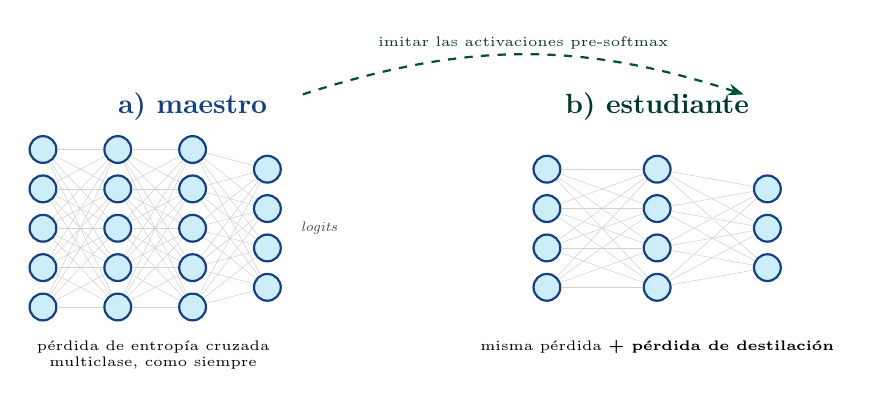
\begin{tikzpicture}[font=\scriptsize,
	nn/.style={circle, draw=UCMNavy, thick, fill=UCMBlue!20, minimum size=3.4mm, inner sep=0pt},
	fl/.style={-{Stealth[length=2mm]}, thick, gray!75}]

	% maestro
	\begin{scope}
		\node[font=\bfseries, text=UCMNavy] at (1.9,2.55) {a) maestro};
		\foreach \i/\y in {0/0, 1/0.5, 2/1.0, 3/1.5, 4/2.0}{
			\node[nn] (t0\i) at (0,\y) {};
			\node[nn] (t1\i) at (0.95,\y) {};
			\node[nn] (t2\i) at (1.9,\y) {};}
		\foreach \i/\y in {0/0.25, 1/0.75, 2/1.25, 3/1.75}{\node[nn] (t3\i) at (2.85,\y) {};}
		\foreach \p in {0,...,4}\foreach \q in {0,...,4}
			{\draw[gray!35, very thin] (t0\p) -- (t1\q); \draw[gray!35, very thin] (t1\p) -- (t2\q);}
		\foreach \p in {0,...,4}\foreach \q in {0,...,3}
			{\draw[gray!35, very thin] (t2\p) -- (t3\q);}
		\node[font=\tiny, anchor=west, text=StanfordGray] at (3.15,1.0) {\emph{logits}};
		\node[font=\tiny, anchor=north, align=center] at (1.4,-0.3)
			{p\'erdida de entrop\'ia cruzada\\ multiclase, como siempre};
	\end{scope}

	% estudiante
	\begin{scope}[xshift=6.4cm]
		\node[font=\bfseries, text=AccentGreen!45!black] at (1.4,2.55) {b) estudiante};
		\foreach \i/\y in {0/0.25, 1/0.75, 2/1.25, 3/1.75}{
			\node[nn] (s0\i) at (0,\y) {};
			\node[nn] (s1\i) at (1.4,\y) {};}
		\foreach \i/\y in {0/0.5, 1/1.0, 2/1.5}{\node[nn] (s2\i) at (2.8,\y) {};}
		\foreach \p in {0,...,3}\foreach \q in {0,...,3}
			{\draw[gray!35, very thin] (s0\p) -- (s1\q);}
		\foreach \p in {0,...,3}\foreach \q in {0,1,2}
			{\draw[gray!35, very thin] (s1\p) -- (s2\q);}
		\node[font=\tiny, anchor=north, align=center] at (1.4,-0.3)
			{misma p\'erdida \textbf{+ p\'erdida de destilaci\'on}};
	\end{scope}

	% flecha de destilación (por encima de los rótulos de cada red)
	\draw[fl, AccentGreen!60!black, dashed] (3.3,2.70) to[out=18, in=162] (8.9,2.70);
	\node[font=\tiny, text=AccentGreen!45!black, anchor=south] at (6.1,3.15)
		{imitar las activaciones pre-softmax};
\end{tikzpicture}
\end{center}
\vspace{0.3em}
\begin{columns}[T]
\begin{column}{6.1cm}
\begin{itemize}
	\item Se entrena una red peque\~na (\emph{estudiante}) para replicar a una grande (\emph{maestro}).
	\item Hinton et al.\ (2015): lo importante es el \textbf{patr\'on de informaci\'on entre clases}, no solo la clase ganadora.
\end{itemize}
\end{column}
\begin{column}{6.1cm}
\begin{itemize}
	\item Zagoruyko \& Komodakis (2017) a\~naden transferencia de atenci\'on: aproximan una ResNet-34 ($\sim$63\,M) con una ResNet-18 ($\sim$11\,M) en ImageNet.
	\item Pero 11\,M sigue siendo m\'as que los $\sim$1\,M de ejemplos de entrenamiento.
\end{itemize}
\end{column}
\end{columns}
\end{frame}

\begin{frame}
\frametitle{¿Alcanza con menos? Discusión}
\footnotesize % ajuste de densidad
\begin{columns}[T]
\begin{column}{6.2cm}
\begin{alertblock}{El estado de la cuestión}
\begin{itemize}
	\item \textbf{No hay demostraciones} de rendimiento de vanguardia en conjuntos complejos con muchos menos par\'ametros que datos de entrenamiento.
	\item Ni la poda ni la destilaci\'on han cambiado ese panorama: los modelos reducidos siguen estando sobreparametrizados.
	\item La evidencia actual sugiere que la sobreparametrizaci\'on \textbf{es necesaria} para generalizar --- al menos para el tama\~no y complejidad de los conjuntos que usamos hoy.
\end{itemize}
\end{alertblock}
\end{column}
\begin{column}{6.0cm}
\begin{exampleblock}{Un giro contraintuitivo}
Bubeck \& Sellke (2021) probaron que en $D$ dimensiones la \textbf{interpolaci\'on suave} exige $D$ veces m\'as par\'ametros que la mera interpolaci\'on.
\vspace{0.3em}

Su conclusi\'on: los modelos actuales para conjuntos grandes como ImageNet \textbf{no est\'an lo bastante sobreparametrizados}. Aumentar a\'un m\'as la capacidad podr\'ia ser la clave para mejorar.
\end{exampleblock}
\vspace{0.3em}
\footnotesize
Queda abierta la pregunta de fondo: ¿es una propiedad \emph{fundamental} de los modelos peque\~nos lo que les impide rendir, o simplemente \textbf{no sabemos entrenarlos}?
\end{column}
\end{columns}
\vspace{0.2em}
\idea{Recordemos la tensi\'on: m\'as par\'ametros hacen el ajuste \emph{m\'as f\'acil} (secci\'on 20.2) y la generalizaci\'on \emph{mejor} (secci\'on 20.4). Separar ambos efectos es justamente lo que a\'un no sabemos hacer.}
\end{frame}

%=====================================================================
\section{¿Tienen que ser profundas?}
%=====================================================================

\begin{frame}
\frametitle{La pregunta que deja abierta el teorema de aproximación universal}
\scriptsize % ajuste de densidad
\begin{columns}[T]
\begin{column}{6.2cm}
\begin{block}{Recordemos}
\footnotesize
El \textbf{teorema de aproximaci\'on universal} dice que una red \emph{superficial} puede aproximar cualquier funci\'on con precisi\'on arbitraria, dadas suficientes unidades ocultas.
\vspace{0.3em}

Entonces, ¿para qu\'e la profundidad?
\end{block}
\vspace{0.2em}
\textbf{Evidencia a favor de la profundidad:}
\begin{itemize}
	\item Hist\'oricamente, el desempe\~no en ImageNet mejor\'o con la profundidad, hasta que entrenar se volvi\'o dif\'icil.
	\item Conexiones residuales y \emph{batch normalization} permitieron ir m\'as profundo, con ganancias proporcionales.
	\item Hoy casi todo el estado del arte (ViT, GPT-3, DALL$\cdot$E-2) usa decenas o cientos de capas.
\end{itemize}
\end{column}
\begin{column}{6.0cm}
\begin{alertblock}{Intentos de ir más superficial}
\footnotesize
\begin{itemize}
	\item Zagoruyko \& Komodakis (2016): ResNets \textbf{m\'as anchas y menos profundas} igualan a ResNet.
	\item Goyal et al.\ (2021): canales convolucionales \textbf{en paralelo} logran un desempe\~no similar con solo \textbf{12 capas}.
	\item Veit et al.\ (2016): en una ResNet lo que manda son los \textbf{caminos cortos de 5--17 capas}.
\end{itemize}
\end{alertblock}
\vspace{0.3em}
\footnotesize
Aun as\'i, el balance de la evidencia dice que la profundidad es cr\'itica: incluso las redes m\'as superficiales con buena clasificaci\'on de im\'agenes necesitan \textbf{m\'as de 10 capas}.
\end{column}
\end{columns}
\vspace{0.2em}
\idea{Sabemos \emph{que} la profundidad hace falta. No sabemos \emph{por qu\'e}.}
\end{frame}

\begin{frame}
\frametitle{Tres explicaciones posibles para la profundidad}
\scriptsize % ajuste de densidad
\begin{columns}[T]
\begin{column}{4.0cm}
\begin{block}{1. Complejidad de la función}
Las redes profundas generan muchas m\'as regiones lineales que las superficiales con los mismos par\'ametros. Existen funciones ``patol\'ogicas'' que requieren exponencialmente m\'as unidades en una red superficial (Eldan \& Shamir, 2016; Telgarsky, 2016).
\vspace{0.3em}

\textcolor{StanfordRed}{\textbf{Pero:}} algunas de esas funciones tampoco se ajustan bien en la pr\'actica con redes profundas (Nye \& Saxe, 2018), y poco indica que las funciones reales sean patol\'ogicas.
\end{block}
\end{column}
\begin{column}{4.0cm}
\begin{block}{2. Tratabilidad del entrenamiento}
Quiz\'a una red superficial \emph{podr\'ia} rendir igual, pero es dif\'icil encontrar una soluci\'on que ajuste \textbf{y} interpole bien.
\vspace{0.3em}

Urban et al.\ (2017) destilaron un conjunto de 16 CNN sobre CIFAR-10 en estudiantes de distinta profundidad: las redes superficiales \textbf{no lograron} replicar al maestro, y el desempe\~no creci\'o con la profundidad \textbf{a igual presupuesto de par\'ametros}.
\end{block}
\end{column}
\begin{column}{4.0cm}
\begin{block}{3. Sesgo inductivo}
Las restricciones de convoluciones y transformers no son generales: procesan localmente y \textbf{integran informaci\'on gradualmente}. Eso es un buen sesgo inductivo, dif\'icil de imponer a una red superficial.
\vspace{0.3em}

Evidencia: la estructura de una CNN \textbf{sin entrenar} ya sirve como prior (Ulyanov et al., 2018); basta entrenar los par\'ametros de BatchNorm con n\'ucleos aleatorios fijos (Frankle et al., 2021); destilar hacia arquitecturas convolucionales funciona mejor que hacia densas.
\end{block}
\end{column}
\end{columns}
\vspace{0.3em}
\idea{Las tres explicaciones son compatibles entre s\'i y ninguna est\'a demostrada. Que el procesamiento local secuencial de una CNN no pueda replicarse f\'acilmente en pocas capas es el argumento m\'as fuerte a favor de la profundidad.}
\end{frame}

%=====================================================================
\section{Cierre}
%=====================================================================

\begin{frame}
\frametitle{Resumen}
\begin{center}
\footnotesize
\begin{tabular}{ll}
\toprule
\textbf{Pregunta} & \textbf{Lo que sabemos}\\
\midrule
¿Por qu\'e se ajustan?      & Sobreparametrizaci\'on y funci\'on de activaci\'on son los dos factores clave\\
¿Importan los datos?        & No: se ajustan p\'ixeles y etiquetas aleatorias igual de bien\\
¿Importa la regularizaci\'on? & Para ajustar, no. Para generalizar, s\'i\\
¿C\'omo es el paisaje?      & Sin m\'inimos locales aparentes; puntos silla arriba, m\'inimos abajo\\
¿C\'omo se llega al m\'inimo? & Por un subespacio de dimensi\'on muy baja, a una familia conexa\\
¿Qu\'e mejora generalizar?  & Sobreparametrizaci\'on, m\'inimos planos, sesgo inductivo, raz\'on lote$/\eta$\\
Doble descenso              & La curva en U cl\'asica es solo la mitad izquierda del dibujo\\
Norma de los pesos          & Ni muy chica ni muy grande: la zona \emph{Goldilocks} explica el \emph{grokking}\\
Robustez                    & Ejemplos adversarios: peque\~nas perturbaciones, cambios dr\'asticos\\
¿Menos par\'ametros?        & Poda y destilaci\'on ayudan, pero siguen sobreparametrizando\\
¿Menos profundidad?         & Parece imprescindible; no hay explicaci\'on definitiva de por qu\'e\\
\bottomrule
\end{tabular}
\end{center}
\end{frame}

\begin{frame}
\frametitle{Lo que todavía no sabemos}
\footnotesize % ajuste de densidad
\begin{center}
\begin{tcolorbox}[colback=StanfordRed!5, colframe=StanfordRed, arc=4pt,
	width=0.95\textwidth, fontupper=\small]
\RaggedRight
\begin{itemize}
	\item No tenemos \textbf{ninguna teor\'ia prescriptiva} que permita predecir en qu\'e circunstancias el entrenamiento y la generalizaci\'on van a funcionar o a fallar.
	\item No conocemos los \textbf{l\'imites} del aprendizaje en redes profundas.
	\item No sabemos si son posibles modelos \textbf{mucho m\'as eficientes}.
	\item No sabemos si, dentro del mismo modelo, existen par\'ametros que \textbf{generalizar\'ian mejor} que los que encontramos.
\end{itemize}
\end{tcolorbox}
\end{center}
\vspace{0.5em}
\begin{block}{Y sin embargo}
El estudio del aprendizaje profundo sigue guiado por \textbf{demostraciones emp\'iricas}. Son innegablemente impresionantes, pero todav\'ia no est\'an acompa\~nadas por una comprensi\'on equivalente de sus mecanismos.
\end{block}
\vspace{0.4em}
\idea{Este es un buen lugar para terminar la unidad: saber usar una herramienta y saber por qu\'e funciona son dos cosas distintas, y en este campo la primera va muy por delante de la segunda.}
\end{frame}

\begin{frame}
\frametitle{Para profundizar}
\begin{itemize}
	\item Prince, \emph{Understanding Deep Learning}, cap.~20 (y cap.~8 sobre doble descenso)\\ \url{https://udlbook.github.io/udlbook/}
	\item Zhang, Bengio, Hardt, Recht \& Vinyals (2017), \emph{Understanding deep learning requires rethinking generalization}, ICLR.
	\item Frankle \& Carbin (2019), \emph{The lottery ticket hypothesis}, ICLR.
	\item Keskar, Mudigere, Nocedal, Smelyanskiy \& Tang (2017), \emph{On large-batch training for deep learning: generalization gap and sharp minima}, ICLR.
	\item Draxler, Veschgini, Salmhofer \& Hamprecht (2018), \emph{Essentially no barriers in neural network energy landscape}, ICML.
	\item Goodfellow, Shlens \& Szegedy (2015), \emph{Explaining and harnessing adversarial examples}, ICLR.
	\item Belkin, Hsu, Ma \& Mandal (2019), \emph{Reconciling modern machine learning practice and the bias-variance trade-off}, PNAS.
\end{itemize}
\vspace{0.3em}
\footnotesize
\textbf{Cuadernos sugeridos (Prince, cap.~20):} 20.1 datos aleatorios, 20.2 gradiente de lote completo, 20.3 billetes de loter\'ia, 20.4 ataques adversarios.
\vspace{0.4em}
\begin{center}
\Large \textbf{¿Preguntas?}
\end{center}
\end{frame}

\end{document}
